% 三种平台对比图
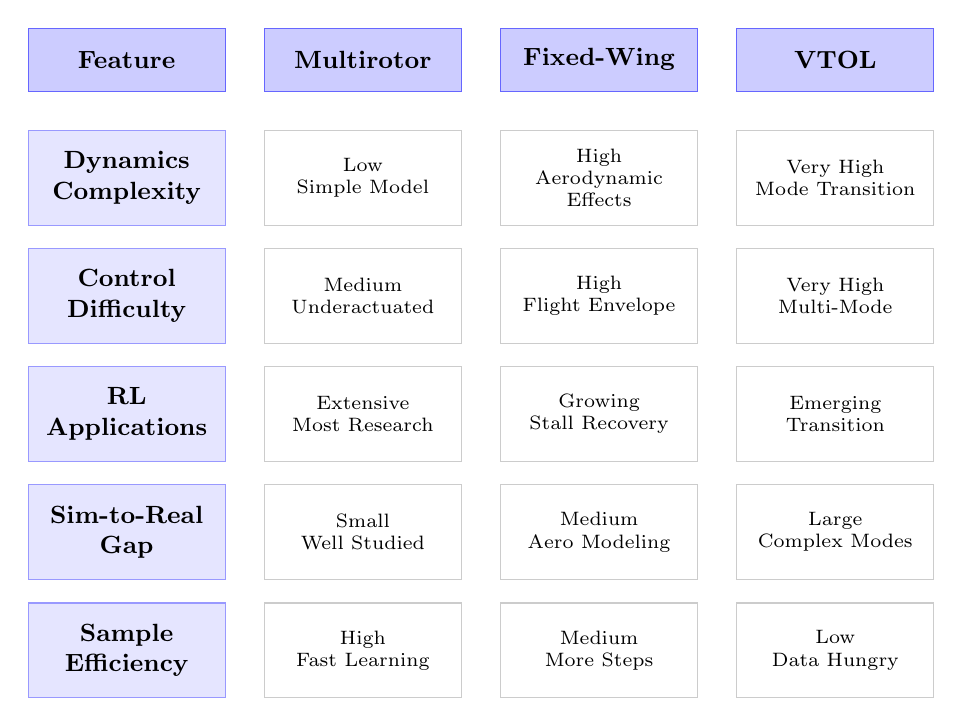
\begin{tikzpicture}[
    node distance=0.6cm,
    header/.style={rectangle, draw=blue!60, fill=blue!20, 
                   minimum width=2.5cm, minimum height=0.8cm, text centered, font=\small\bfseries},
    cell/.style={rectangle, draw=gray!40, fill=white,
                 minimum width=2.5cm, minimum height=1.2cm, text centered, font=\scriptsize, align=center},
    rowheader/.style={rectangle, draw=blue!40, fill=blue!10,
                      minimum width=2.5cm, minimum height=1.2cm, text centered, font=\small\bfseries, align=center}
]

% Headers
\node[header] (h1) at (0,0) {Feature};
\node[header] (h2) at (3,0) {Multirotor};
\node[header] (h3) at (6,0) {Fixed-Wing};
\node[header] (h4) at (9,0) {VTOL};

% Row 1: Complexity
\node[rowheader] (r1h) at (0,-1.5) {Dynamics\\Complexity};
\node[cell] (r1c1) at (3,-1.5) {Low\\Simple Model};
\node[cell] (r1c2) at (6,-1.5) {High\\Aerodynamic\\Effects};
\node[cell] (r1c3) at (9,-1.5) {Very High\\Mode Transition};

% Row 2: Control Difficulty
\node[rowheader] (r2h) at (0,-3) {Control\\Difficulty};
\node[cell] (r2c1) at (3,-3) {Medium\\Underactuated};
\node[cell] (r2c2) at (6,-3) {High\\Flight Envelope};
\node[cell] (r2c3) at (9,-3) {Very High\\Multi-Mode};

% Row 3: RL Applications
\node[rowheader] (r3h) at (0,-4.5) {RL\\Applications};
\node[cell] (r3c1) at (3,-4.5) {Extensive\\Most Research};
\node[cell] (r3c2) at (6,-4.5) {Growing\\Stall Recovery};
\node[cell] (r3c3) at (9,-4.5) {Emerging\\Transition};

% Row 4: Sim-to-Real
\node[rowheader] (r4h) at (0,-6) {Sim-to-Real\\Gap};
\node[cell] (r4c1) at (3,-6) {Small\\Well Studied};
\node[cell] (r4c2) at (6,-6) {Medium\\Aero Modeling};
\node[cell] (r4c3) at (9,-6) {Large\\Complex Modes};

% Row 5: Sample Efficiency
\node[rowheader] (r5h) at (0,-7.5) {Sample\\Efficiency};
\node[cell] (r5c1) at (3,-7.5) {High\\Fast Learning};
\node[cell] (r5c2) at (6,-7.5) {Medium\\More Steps};
\node[cell] (r5c3) at (9,-7.5) {Low\\Data Hungry};

\end{tikzpicture}
